%%%%%%%%%%%%%%%%%%%%%%%%%%%%%%%%%%%%%
%% Master Thesis - Computer Engineering
%% Copyright 2009 Ricardo Alexandre Fiorelli, Erick Poletto
%% This document is distributed by the terms of the license
%% included in the file LICENCE.
%%%%%%%%%%%%%%%%%%%%%%%%%%%%%%%%%%%%%

%%%%%%%%%%%%%%%%%%%%%%%%%%%%%%%%%%%%%
%% Second Chapter
%% State of the Art
%%%%%%%%%%%%%%%%%%%%%%%%%%%%%%%%%%%%%

\chapter{State of the Art} \label{chap2:state_of_the_art}
    In terms of hardware and equipment, the main measures to be taken towards a Green ICT environment can be grouped in the following categories:%XXX
    \begin{itemize}
        \item Workstation Configuration;
        \item Policies / Tools / Labels;
        \item Thin client architectures;
        \item Servers and Virtualization;
        \item Data Storage;
        \item Power Architectures;
        \item Data Center Infrastructure.
    \end{itemize}
    
    For each of those categories there are several types of information that are relevant to the evaluation of the intervention and their consequent energy savings. For each one a list of possible interventions will be made, and after that analyzed if they are either purely conceptual or available in the market. Moreover, it is important to know exactly where the power is going and where the energy is being wasted. In hands with that information, it is possible to redirect it to the places with more necessity and ameliorate the computers with more idle time, by applying one of the above categories before. Therefore, it is feasible to draw a more realistic figure of what is going on with the energy consumed in the place.
    
    It is possible to compare how much energy is spent by three types of components, Computers on Table~\ref{tab:energy_used_computer}, Monitors on Table~\ref{tab:energy_used_monitor} and an Apple on Table~\ref{tab:energy_used_apple_20}.
    \begin{table}
        \centering
        \begin{tabular}{|c|c|}
        \hline
        \multicolumn{ 2}{|c|}{{\bf Computers}} \\
        \hline
        Desktop Computer & 60-250 watts \\
        \hline
        On screen Saver$^a$ & 60-250 watts \\
        \hline
        Sleep / Standby & 1-6 watts \\
        \hline
        Laptop & 15-45 watts \\
        \hline
        \end{tabular}\linebreak
        $^a$ no difference
        \captionof{table}{Energy used by a standard computer} 
        \label{tab:energy_used_computer}
    \end{table}
    \begin{table}
        \centering
        \begin{tabular}{|c|c|}
        \hline
        \multicolumn{ 2}{|c|}{{\bf Monitors}} \\
        \hline
        Typical 17" CRT &   80 watts \\
        \hline
        Typical 17" LCD &   35 watts \\
        \hline
        Apple MS 17" CRT$^a$ &   63 watts \\
        \hline
        Apple MS 17" CRT$^b$ &   54 watts \\
        \hline
        Screen saver$^c$ & same as above \\
        \hline
        Sleeping monitor$^d$ & 0-15 watts \\
        \hline
        Monitor turned off at switch & 0-10 watts \\
        \hline
        \end{tabular}  \linebreak
        $^a$ mostly white (blank IE window) \linebreak
        $^b$ mostly black (black Windows desktop with just a few icons)\linebreak
        $^c$ any image on screen\linebreak
        $^d$ dark screen
        \captionof{table}{Energy used by Monitors} 
        \label{tab:energy_used_monitor}
    \end{table}
    \begin{table}
        \centering
        \begin{tabular}{|c|c|}
        \hline
        \multicolumn{ 2}{|c|}{{\bf Apple iMac G5 with built in 20" LCD screen}} \\
        \hline
              Idle &   97 watts \\
        \hline
        Monitor dimmed &   84 watts \\
        \hline
        Monitor sleep &   62 watts \\
        \hline
        Copying files &  110 watts \\
        \hline
        Watching a DVD &  110 watts \\
        \hline
        Opening a lot of pictures &  120 watts \\
        \hline
        Computer sleep &  3.5 watts \\
        \hline
        \end{tabular}  
        \captionof{table}{Energy used by Apple iMac G5 with built in 20" LCD screen} 
        \label{tab:energy_used_apple_20}
    \end{table}
    
    \section{Computer Energy Management Categories} \label{sec2:energy_categories}
    % TODO
    %/***********Seria legal se fosse feita uma conclus�o para cada categoria*************/
    
    \subsection{Workstation Configuration}\label{sec2:workstation_configuration}
        This category represents the components used in a certain machine configuration. All the information about each component performance and power consumption can be obtained from several sources, such as the manufacturer specifications, benchmarks or direct measurements in the case of energy consumption
        Listed below are the necessary information to evaluate interventions and their energy savings:
            \paragraph*{Single-core / Multi-core processors}
            \paragraph*{CPU Type}
            \paragraph*{Type and dimension of RAM memory}
            \paragraph*{Type and dimension of cache memory}
            \paragraph*{Chassis (power supply, fan)}
            \paragraph*{Monitor type} It is important to say that using flat panel liquid crystal display (LCD) monitors and not conventional CRT monitors can reduce energy consumption by a third. LCD monitors also run cooler, which helps save on air conditioning costs. In addition to that, selecting the right-sized monitor to meet the needsof the user helps, because the bigger the monitor, the more energy it uses.
            \paragraph*{Hard drives (number and type)}
            \paragraph*{Auto-sleep, remote sleep and screen saver} Enabling the energy saving settings on PCs and peripherals is also valuable act, due to the fat that a computer in idle mode uses 20 to 50 times the power of a computer in standby mode. For example, when the computer is in standby mode the computer uses 0 to 6 watts. Reducing the time delay in which the computer will enter in the power saving mode is also a good thing to be done. Another thing to be done, is to disable the screen saver. Studies shown that a monitor in screen saving mode uses significantly more energy than in standby mode.
            \paragraph*{Efficiency benchmarks fat/thin}
            \paragraph*{Performance benchmarks}
            \paragraph*{Overall and single components power consumption benchmarks, in several load conditions (idle, SO, main applications)}
            \paragraph*{Trade off between performance and consumption}

    \subsection{Policies / Tools / Labels} \label{sec2:policies_tools_labels}
        The amount of saved energy depends also on technology acquisition and managerial policies. There are a number of specialized tools that may be used in order to help enforcing these policies and tools. 

        These policies can be made as acquisition of new computers or components labeled as green by the manufacturer, purchase of dual or multi-core processors, or even the discourage of purchasing or use of other parts, such as dual or large monitors. Likewise, other kinds of policies are a good idea to be defined, and they concern in the use of the workstation, for instance, to turn off the computer if they are going to be unused for a long time, shutdown over nights, and others. These policies, or rules, are important either to enforce the company's position through the green idea either to keep track of the list of thing yet to be prepared in order to convert the computers and workers as green as possible.
        
        Furthermore, the use of tools that automates these methods is welcome to the enterprise. There are many tools, which let the computer in standby mode, or even turn off after a long period of no utilization. In addition, the use of networked pieces of hardware can be an effective way to achieve the green. Additionally, networked systems allow several nearby users to share a single (faster) printer generally save time, cost, and energy compared with each computer having a dedicated printer, it will decrease their idle time and provide for more cost-effective use of the equipment. Above that, choosing multifunction devices (MFD) that do the work that used to require several machines. In addition to saving space and materials, these All-in-Ones save energy compared to several products working in parallel. Select printers or multifunction products that offer two-sided printing to reduce paper and energy usage. The Table~\ref{tab:energy_recommendation_efficient_printer}\footnote{\url{http://www1.eere.energy.gov/femp/procurement/eep_printer.html}} describes the characteristics that am energy-efficient networked printer should have, in relation to the number of pages per minute it prints. 
        
        \begin{table}
        \centering
            \begin{tabular}{|r|c|c|}
            \hline
            \multicolumn{ 3}{|c|}{{\bf Efficiency Recommendation}} \\
            \hline
            \multicolumn{ 1}{|c|}{Printer Speed} & \multicolumn{ 2}{|c|}{Recommended ``Sleep'' Mode$^a$} \\
            \hline
            \multicolumn{ 1}{|c|}{} & Laser B/W + All Ink jet$^b$ & Laser Color$^c$ \\
            \hline
            $\geq$10 pages/min & 10 watts or less & 35 watts or less \\
            \hline
            11-20 pages/min & 20 watts or less & 45 watts or less \\
            \hline
            21-30 pages/min & 30 watts or less & 70 watts or less \\
            \hline
            31-44 pages/min & 40 watts or less & 70 watts or less \\
            \hline
            $>$44 pages/min & 75 watts or less & 70 watts or less \\
            \hline
            \end{tabular}\linebreak            
            $^a$ ``Sleep'' mode is a low-power standby condition, it restores automatically with a print request.\linebreak            
            $^b$ Includes both black-ink and color ink jets, and printer/fax combinations.\linebreak            
            $^c$ Also includes LED and thermal transfer color printers.
            \captionof{table}{Energy Recommendation to an Energy-Efficient Printer} \label{tab:energy_recommendation_efficient_printer}
        \end{table}
        
        Besides these facts, it is also a choice to buy only eco-labeled products. Eco-label is a category given to products, which comply some of the energy efficiency specifications provided by the owner companies of these labels. The most famous of these labels is the ENERGY STAR$^{\textcircled {\scriptsize R}}$, which is a voluntary energy efficiency program sponsored by the U.S. Environmental Protection Agency. For example, An ENERGY STAR$^{\textcircled {\scriptsize R}}$ qualified computer is possible to use up to 70\% less electricity than computers without enabled power management features.
            
        \subsection{Thin Clients Architectures} \label{sec2:thin_clients}
            O que sao thin clients\ldots
            
            \subsubsection*{PC vs. Thin Client: Performance}
                In order to analyze and give a base for a comparison of the performance between standard PCs and two types of thin clients, a set of tests were executed, on networks varying the number of active clients, each running the same typical office applications tasks. The following client platforms participated in this study:
                \begin{itemize}
                    \item PC: OptiPlex 210L PCs, basic managed PC desktops running Windows XP Professional;
                    \item Sun thin client: Sun Ray 2 running Sun Ray proprietary software;
                    \item Wyse thin client: Wyse Winterm 5150SE, Linux-based thin clients running Wyse Linux V6.
                \end{itemize}
                Each network used a standard file server, an HP ProLiant DL360 3.4MHz with and Intel Xeon processor and Microsoft Server 2003 Enterprise Edition. For test reasons, all files were manipulated by the PC were stored at the server. The tests are listed below:
                \begin{itemize}
                    \item Calculating subtotal in Microsoft Office Excel 2003 (Figure~\ref{fig:graphic_excel_test} and Table~\ref{tab:table_excel_test})
                    \item Compressing a PDF within Adobe Acrobat 7.0 Standard (Figure~\ref{fig:graphic_pdf_test} and Table~\ref{tab:table_pdf_test})
                \end{itemize}
                
                \begin{figure}[h!tb]
                    \centering
                    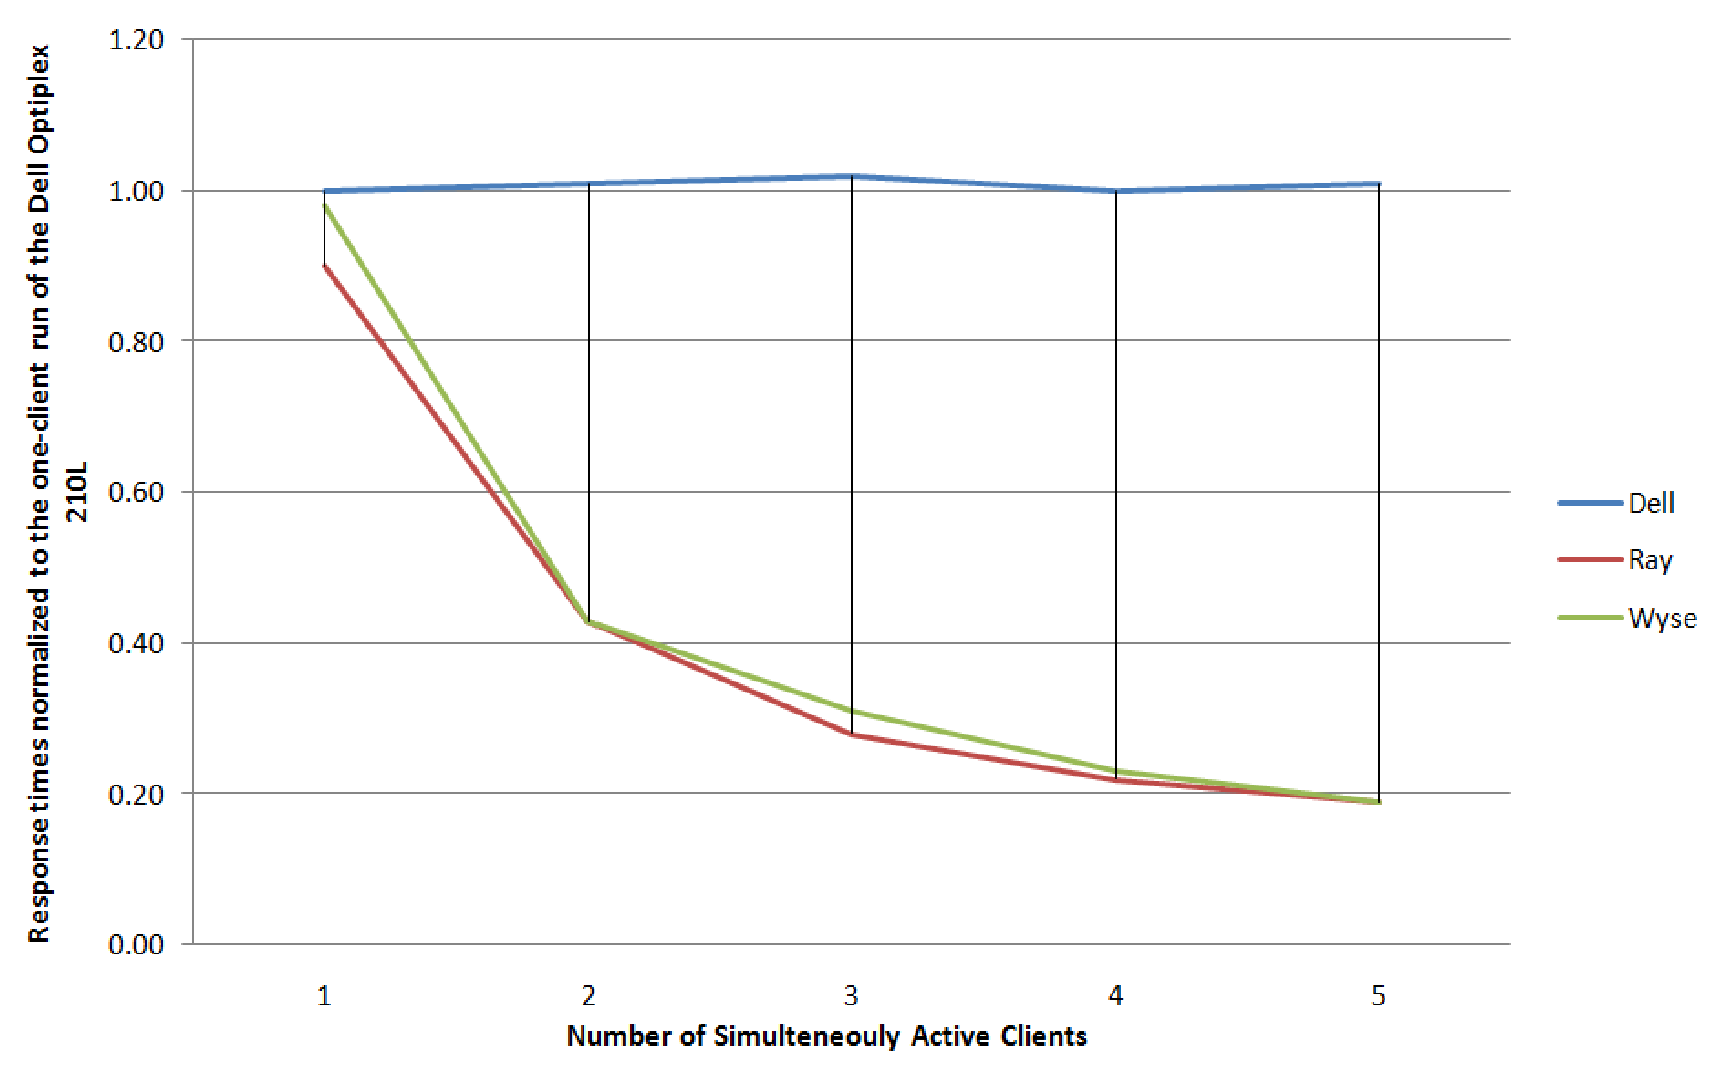
\includegraphics[scale=0.5]{graphics/graphic_excel_test}
                    \caption{Normalized Excel Subtotals Task Response Times}
                    \label{fig:graphic_excel_test}
                \end{figure}
                \begin{table}
                    \centering
                    \begin{tabular}{|c|c|c|c|c|c|c|}
                    \hline
                    \multicolumn{ 3}{|c|}{Performance Results} &            & \multicolumn{ 3}{|c|}{Comparative Rating} \\
                    \hline
                    PC solution & \multicolumn{ 2}{|c|}{Thin-client solutions} & Number of   & PC solution & \multicolumn{ 2}{|c|}{Thin-client solutions} \\
                    \hline
                          Dell &        Sun &       Wyse & concurrent &       Dell &        Sun &       Wyse \\

                      OptiPlex &        Ray &    Winterm &     active &   OptiPlex &        Ray &    Winterm \\

                          210L &          2 &     5150SE &    clients &       210L &          2 &     5150SE \\
                    \hline
                          12.9 &       13.2 &       13.1 &          1 &       1.00 &       0.90 &       0.98 \\
                    \hline
                          12.8 &       30.2 &       29.7 &          2 &       1.01 &       0.43 &       0.43 \\
                    \hline
                          12.7 &       45.5 &       41.9 &          3 &       1.02 &       0.28 &       0.31 \\
                    \hline
                          12.9 &       58.3 &       57.3 &          4 &       1.00 &       0.22 &       0.23 \\
                    \hline
                          12.8 &       68.1 &       67.9 &          5 &       1.01 &       0.19 &       0.19 \\
                    \hline
                    \end{tabular}  
                    \captionof{table}{Performance Results for Excel Subtotals Calculation} 
                    \label{tab:table_excel_test}
                \end{table}
                \begin{figure}[h!tb]
                    \centering
                    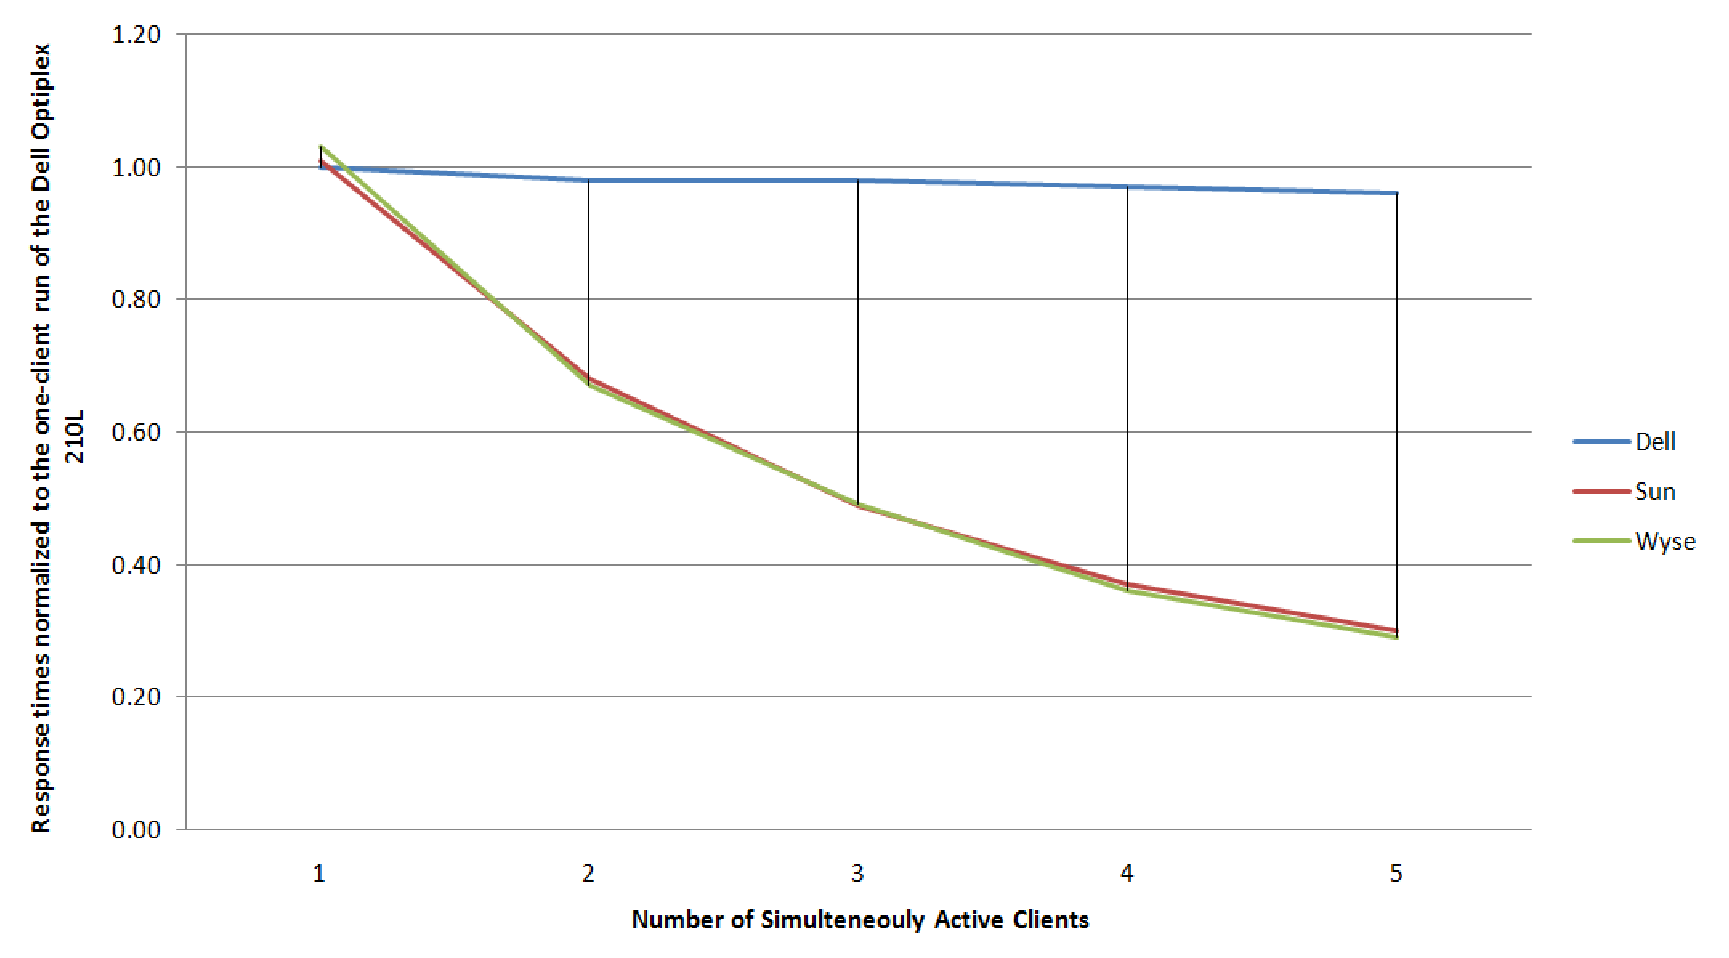
\includegraphics[scale=0.5]{graphics/graphic_pdf_test}
                    \caption{Normalized PDF Subtotals Task Response Times}
                    \label{fig:graphic_pdf_test}
                \end{figure}
                \begin{table}
                    \centering
                    \begin{tabular}{|c|c|c|c|c|c|c|}
                    \hline
                    \multicolumn{ 3}{|c|}{Performance Results} &            & \multicolumn{ 3}{|c|}{Comparative Rating} \\
                    \hline
                    PC solution & \multicolumn{ 2}{|c|}{Thin-client solutions} & Number of   & PC solution & \multicolumn{ 2}{|c|}{Thin-client solutions} \\
                    \hline
                        Dell   &        Sun &       Wyse & concurrent &     Dell   &        Sun &       Wyse \\

                      OptiPlex &        Ray &    Winterm &     active &   OptiPlex &        Ray &    Winterm \\

                          210L &          2 &     5150SE &    clients &       210L &          2 &     5150SE \\
                    \hline
                          16.1 &       16.0 &       15.6 &          1 &       1.00 &       1.01 &       1.03 \\
                    \hline
                          16.4 &       23.8 &         24 &          2 &       0.98 &       0.68 &       0.67 \\
                    \hline
                          16.5 &       33.0 &       33.1 &          3 &       0.98 &       0.49 &       0.49 \\
                    \hline
                          16.6 &       43.7 &       44.3 &          4 &       0.97 &       0.37 &       0.36 \\
                    \hline
                          16.7 &       54.0 &       55.1 &          5 &       0.96 &       0.30 &       0.29 \\
                    \hline
                    \end{tabular}  
                    \captionof{table}{Performance Results for PDF Compression Subtotals Calculation}
                    \label{tab:table_pdf_test}
                \end{table}
                \pagebreak
                
            \subsubsection*{PC vs. Thin Client: Power Consumption}
                Supposing 30 thin users share a 400W server, the total power consumption will be 1300W - a yearly cost of \euro640.00. 30 PCs would consume 10000W instead - a yearly cost of \euro4900.00 (assuming the MWh cost is \euro80.00). The Table~\ref{tab:pc_thin_client_power_consumption} shows the power consumption of thin-client and PC.
                \begin{table}
                \centering
                    \begin{tabular}{|c|c|c|}
                    \hline
                        {\bf } & {\bf Thin Client} &   {\bf PC} \\
                    \hline
                    {\bf Weight} & 2.2 - 7.7 lbs & 22 - 33 lbs \\
                    \hline
                    {\bf Volume} & 1.5 - 3 dm$^3$ & 30 - 35 dm$^3$ \\
                    \hline
                    {\bf Packing material} & 2.2 - 4.4 lbs &   3 - 5 kg \\
                    \hline
                    {\bf Power consumption\linebreak (including monitor)} & 20 - 50 watt & 300 - 400 watt \\
                    \hline
                    {\bf Heat rejection} & 5 - 35 watt & 85 - 115 watt \\
                    \hline
                    {\bf Noise level} & 0 dbA & 50 - 60 dbA \\
                    \hline
                    \end{tabular}  
                    \captionof{table}{PC and thin client power consumption} 
                    \label{tab:pc_thin_client_power_consumption}
                \end{table}
                
            \subsubsection*{Hardware Savings}
                \paragraph*{Savings on client hardware} 
                    The economy brought by the substitution of PCs with thin clients was estimated around US\$ 208 per PC per year. The estimative considered the average prices of a PC, an adequate thin client and the PC upgrade costs every 3 years. If energy consumption is considered, the savings will be even greater.

                The following considerations were taken:
                \begin{itemize}
                    \item Thin client cost: US\$250.00 x PC cost: US\$750.00;
                    \item PC needs to be upgraded every 3 years and thin clients need to be replaced every 6 years.
                \end{itemize}
                Therefore, in a 6-year period US\$1500.00 will be spent on a PC against \$250.00 that will be spent on a thin client.

            \paragraph*{Extra server hardware costs}
                Considering that:
                \begin{itemize}
                    \item On average 30 users will need a dual processor server with 4 GB of RAM and SCSI hard disks;
                    \item A brand new server should cost around US\$4,500.00 and will depreciate on average in 3 years.
                \end{itemize}
                For 60 users, the thin client solution should out-price the PC one by US\$11,300.00 per year, excluding the administration costs of both solutions.

        \subsection{Servers and Virtualization} \label{sec2:servers_virtualization}
            bla bla bla\ldots
            
            \subsubsection*{Rack vs. Blade}
                According to Goldworm\cite{barbAnne07}, Blade servers are a package of ``ultra-high density components including servers, storage, and communications interfaces in a pre-wired chassis with shared components such as power, cooling, and networking. In contrast to the conventional \emph{horizontal} positioning within a rack (rack mounted servers), blades are typically (though not always) installed \emph{vertically} in a blade chassis, like books in a bookshelf''. This disposition of the servers provide a high density of the components and thus performance, for example, 60 blade servers can fit in the same physical space as 42 rack-mounted servers. Another improvement reached with this type of server is the integration of a remote system management, differently form the ordinary (rack or standalone), where it is an add-on. An example of this type of server can be seen on Figure~\ref{fig:example_blade_server}. Moreover, Blade servers\footnote{\url{http://ieeexplore.ieee.org/xpl/freeabs_all.jsp?tp=&arnumber=1362591&isnumber=29851}} are computer servers designed to minimize the use of physical space. A blade enclosure, which can hold from 8 to 24 \cite{Rehn08} blade servers, provides common services such as power supply, cooling and networking thus eliminating redundancies in each individual blade server. More than 250 blade servers can be easily accommodated in a single rack. On the other hand approximately 42 servers can be accommodated to a standard rack when it comes to the other lower end servers available in the market. Whereas, rack-mounted servers are those arrange in industrial rack. A single rack is capable of holding 10 to 20 servers. Therefore, this type of servers come with rails or slides to ease inserting and removing of the components\cite{Bailey09}.
            \begin{figure}[h!tb]
                \centering
                \subfloat[IBM LS20]{
                    \label{fig:ibm_ls20_blade_server}
                    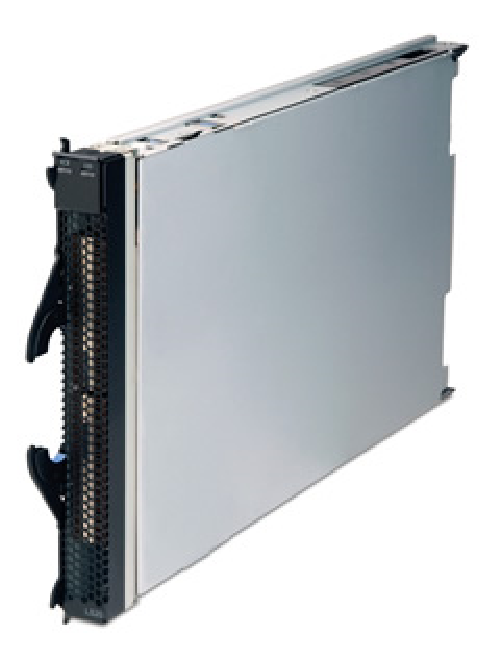
\includegraphics[width=0.3\textwidth]{graphics/ibm_ls20_blade_server}}
                \subfloat[Sun 6000 Series Blade Enclosure]{
                    \label{fig:sun_6000_blade_enclosure}
                    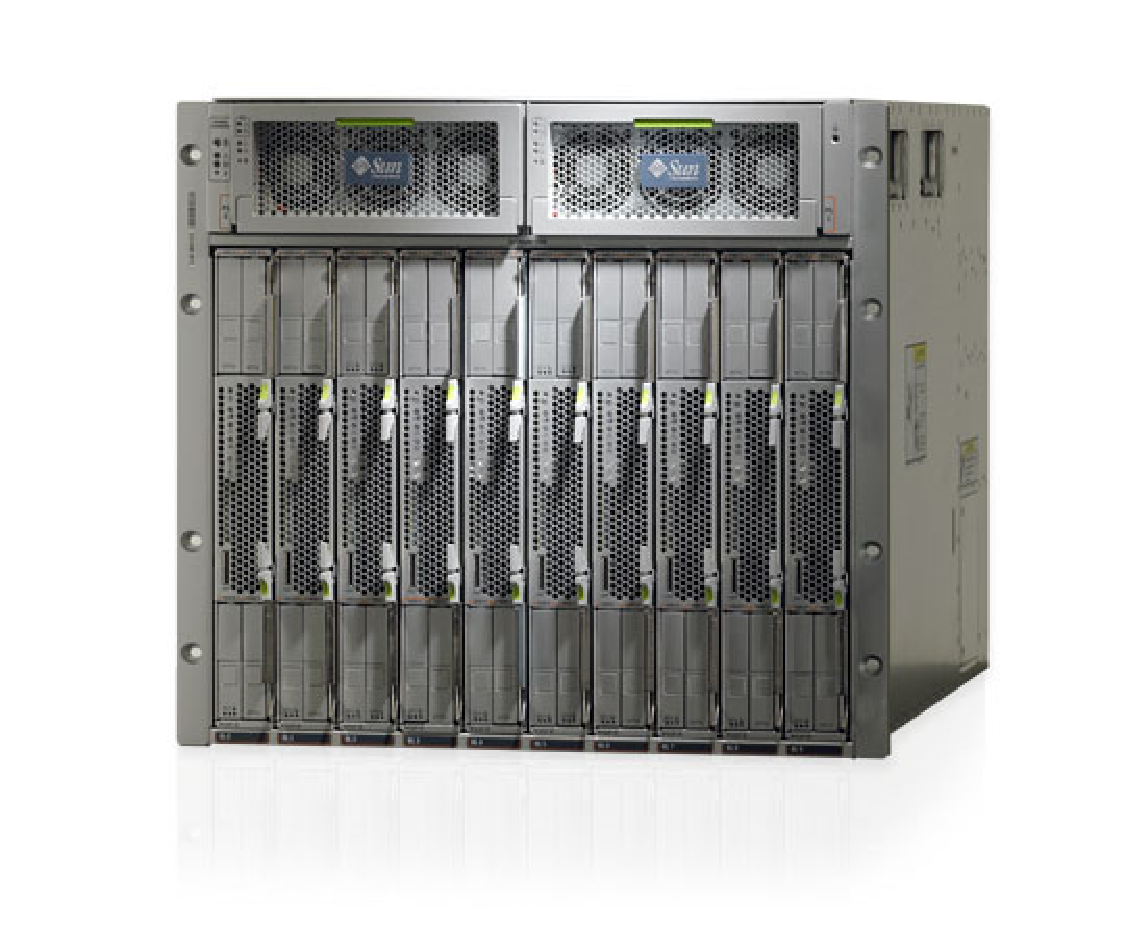
\includegraphics[width=0.3\textwidth]{graphics/sun_6000_blade_enclosure}}
                \subfloat[HP Intros Rack]{
                    \label{fig:hp_intros_blade_server_rack}
                    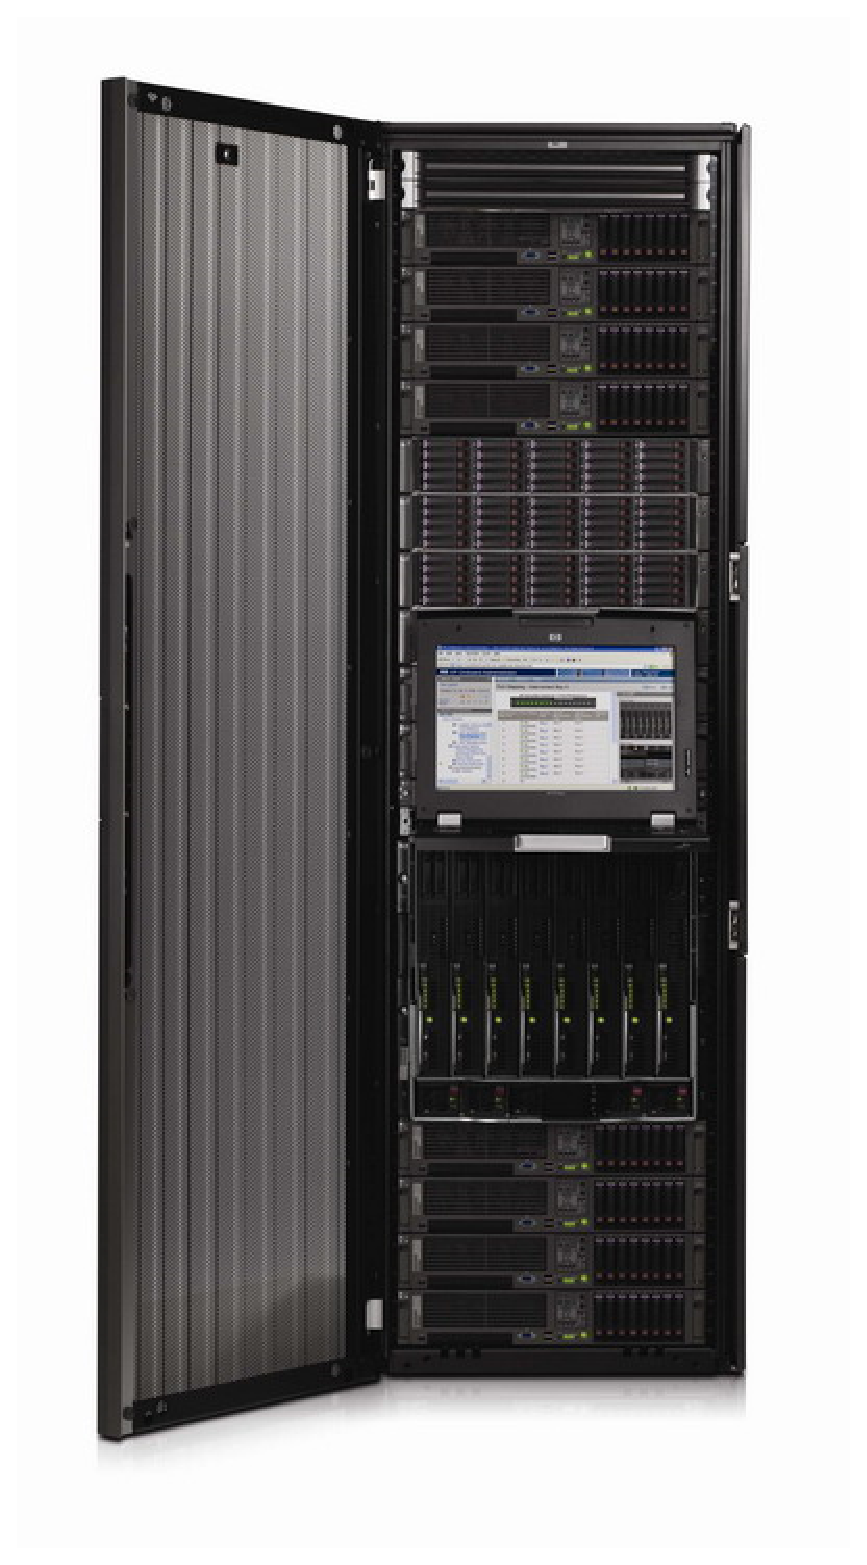
\includegraphics[width=0.3\textwidth]{graphics/hp_intros_blade_server_rack}}
                \caption{Examples of Blade Servers}
                \label{fig:example_blade_server}
            \end{figure}
            \begin{figure}[h!tb]
                \centering
                \subfloat[Chenbro 5U RM51924]{
                    \label{fig:chenbro_5urm51924}
                    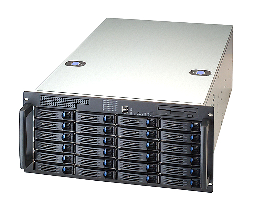
\includegraphics[width=0.3\textwidth]{graphics/chenbro_5U_RM51924}}
                \subfloat[Rack Server]{
                    \label{fig:rack_server}
                    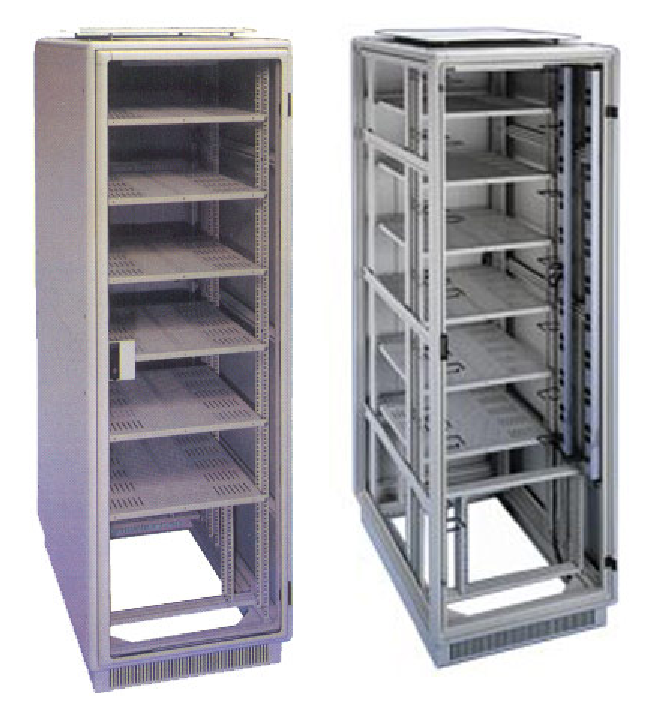
\includegraphics[width=0.3\textwidth]{graphics/rack_server}}
                \caption{Examples of Rack Servers}
                \label{fig:example_rack_server}
            \end{figure}
            In the Table~\ref{tab:power_consumption_several_servers}, a comparison is made between IBM HS21 blades and x3550 rack servers. The blades and rack servers have comparable performance.
            \begin{itemize}
                \item 2.0 GHz intel quad core;
                \item 8 GB DDR2 memory;
                \item Both in standard configuration, with no HDDs.
            \end{itemize}
            \begin{table}
                \centering
                \begin{tabular}{|c|c|c|c|}
                \hline
                \multicolumn{ 1}{|c|}{{\bf IBM server model}} & \multicolumn{ 1}{|c|}{{\bf Base Power}} & \multicolumn{ 1}{|c|}{{\bf kWh consumed}} & \multicolumn{ 1}{|c|}{{\bf Total cost }} \\
                \multicolumn{ 1}{|c|}{{\bf }} & \multicolumn{ 1}{|c|}{{\bf Consumption}} & \multicolumn{ 1}{|c|}{{\bf over 5 years}} & \multicolumn{ 1}{|c|}{{\bf (\$0.03/kWh)}} \\
                \multicolumn{ 1}{|c|}{{\bf }} & \multicolumn{ 1}{|c|}{{\bf }} & \multicolumn{ 1}{|c|}{{\bf }} & \multicolumn{ 1}{|c|}{{\bf over 5 years}} \\
                \hline
                BC-H Chassis, no blades & 0.510 kWh &     22,350 &  \$670.50  \\
                \hline
                BC-H HS21 blade & 0.318 kWh &     13,936 &  \$418.08  \\
                \hline
                x3550 server & 0.373 kWh &     16,346 &  \$490.39  \\
                \hline
                x3650 server & 0.455 kWh &     19,940 &  \$598.20  \\
                \hline
                BC-H chassis with 14 & 4.962 kWh &    217,455 & \$6,523.65  \\
                HS21 blades &  &  &  \\
                \hline
                14 x3550 servers & 5.222 kWh &    228,849 & \$6,865.46  \\
                \hline
                14 x3650 servers & 6.370 kWh &    279,259 & \$8,374.80  \\
                \hline
                \end{tabular}  
                \captionof{table}{Power consumption for several servers, excluding cooling and redundancy}%XXX colocar referencia
                \label{tab:power_consumption_several_servers}
            \end{table}
            Thus, a possible conclusion to this comparison is that with Blade servers the gain with space, performance and, more importantly, power consumption is much smaller than with Rack-mounted devices.
            \begin{itemize}
                \item Space saving and efficiency - packaging more computer power in a significantly smaller area;
                \item Consolidation of servers to improve and centralize management as well as utilization;
                \item Return on investment (ROI) and improved total cost of ownership (TOC) through increased hardware utilization and reduced operating expenses;
                \item More energy efficient, due to existence of centralized power supply, cooling and networking.
            \end{itemize}
            According to the figures, the choice of using a blade server provides roughly 5\% power saving over a similar rack-mount configuration. The main benefit brought by the use of blade servers, however, is the processing density, as a rack filled with blade servers may carry up to 50\% more servers than one with rackable servers. Other benefits are that blade servers are easier to service and reduce the number of power cables needed from as many as 80\% \cite{Hendenson07}. 
            
            However, the high power density might prove to be a problem to server farms in terms of overheating\footnote{---- falar disso na parte de cooling}.
            
            \subsubsection*{Virtualization}
                There are two kinds of virtualization that may be used in a data center: storage and computing virtualization.
                \begin{description}
                    \item[Storage Virtualization] %XXX
                    \item[Computing Virtualization] %XXX
                \end{description}
                
                
        \subsection{Data Storage} \label{sec2:data_storage}
        
        
        \subsection{Power Architectures} \label{sec2:power_architectures}
        
        
        \subsection{Data Center Infrastructure} \label{sec2:data_center_infrastructure}
            


\section{Green ICT} \label{sec2:green_ict}
% TODO
\section{Devices Consumption} \label{sec2:devices_consumption} 
% TODO
\section{Measurement Tools} \label{sec2:tools}
% TODO
